\documentclass[a4paper]{article}
\usepackage{float}
\usepackage[ruled,vlined,linesnumbered,algo2e]{algorithm2e}
\usepackage{amsmath,amssymb}
\usepackage{makecell}
\usepackage{tikz}
\usepackage[margin=0.8in]{geometry}
%\usepackage{biblatex} %Imports biblatex package
%\addbibresource{NLA.bib}
\DeclareMathOperator*{\argmax}{arg\,max}
\DeclareMathOperator*{\argmin}{arg\,min}
\DeclareMathOperator*{\diag}{diag}
\DeclareMathOperator*{\trace}{trace}
\DeclareMathOperator*{\sign}{sign}

\newcommand*\circled[1]{\tikz[baseline=(char.base)]{
		\node[shape=circle,draw=red,inner sep=1pt] (char) {#1};}}
\newcommand{\mbf}[1]{\mathbf{#1}}
\setlength\parindent{0pt} %% Do not touch this
\usepackage{amsthm}
\newtheorem{lemma}{Lemma}
\newtheorem{theorem}{Theorem}
%% -----------------------------
%% TITLE
%% -----------------------------
\title{Homework: Regularization} %% Assignment Title
%% Change "\today" by another date manually
%% -----------------------------
%% -----------------------------

%% %%%%%%%%%%%%%%%%%%%%%%%%%
\newcommand\myemptypage{
	\null
	\thispagestyle{empty}
	\addtocounter{page}{-1}
	\newpage
}

\usepackage{fancyhdr}
\usepackage{listings}
%\usepackage{siunitx}
\usepackage{hyperref}
\usepackage{etoolbox,refcount}
\usepackage{multicol}
\usepackage{tabularx,colortbl}
\usepackage{lastpage}
\usepackage{pgfplots}
\pgfplotsset{compat = newest}
\usepackage{biblatex} %Imports biblatex package
%\addbibresource{NLA.bib}
\usepackage{diagbox}
\pagestyle{fancy}
\usepackage{caption}
\usepackage{subcaption}
\usepackage{mathtools}
\usepackage{cleveref}
\usepackage[bottom]{footmisc}
\usepackage{comment}

\fancyhead[C]{}
\fancyhead[r]{}
%\renewcommand{\footrulewidth}{1pt}
\fancyfoot[L]{}
\fancyfoot[C]{}
\fancyfoot[R]{\thepage\ / \pageref*{LastPage}}

\begin{document}
	
	\begin{titlepage}
		
		\newcommand{\HRule}{\rule{\linewidth}{0.5mm}}  
		
		\begin{center}
			
			%\includegraphics[scale=0.3]{Documents/KUL_ENG.png}\\[1cm]
			\textsc{\LARGE Faculty of Engineering Science}\\[1.5cm] 
			
			
			\HRule \\[0.1cm]
			
			{\huge{ \bfseries Denoising and inpainting with wavelets}} 
			\vspace{5pt}
			{\\ \Large{\bfseries Wavelets with application in signal and Image processing}}
			\HRule \\[1cm]
			
			%\includegraphics[width=0.3\textwidth]{images1/INEOS.png}\\
			\vspace*{0.1cm}
			
			\begin{minipage}{0.4\textwidth}
				\textit{Auteur}
				\begin{flushleft} \large
					\begin{enumerate}
						\item[] \textsc{Thakur} Arnav\\
                        \item[] \textsc{Mohamed Yassin} Arman\\

						
					\end{enumerate} 
				\end{flushleft}
			\end{minipage}\\[1cm]
			\begin{minipage}{0.4\textwidth}
				\textit{Professors}
				\begin{flushleft}
					\begin{enumerate}
						\item[] Prof. Daan Huybrechs\\
					\end{enumerate} 
				\end{flushleft}
			\end{minipage}\\
			
			\vspace*{1.5cm}
			
			
\includegraphics[width=0.5\textwidth]{Images/KUL_Eng_logo.png}\\
			{\Large{Academic year 2023 - 2024}}
			
		\end{center}
	\end{titlepage}
	
	\newpage
	
	\tableofcontents
	
	\newpage

    \section{Wavelet-based denoising}
 
	\subsection{A univariate functions with noise}

    \subsubsection{Question 2.1}

    Function being sampled, $N=1000$, between $[-2,2]$
    \begin{equation*}
        f(x) = (2+\cos{(x)}) |x| \sign{(x-1)}
    \end{equation*}
    
    Tested for wavelet transform of 4 levels deep, using the Daubechies 2 
    \begin{figure}[H]
	\centering
	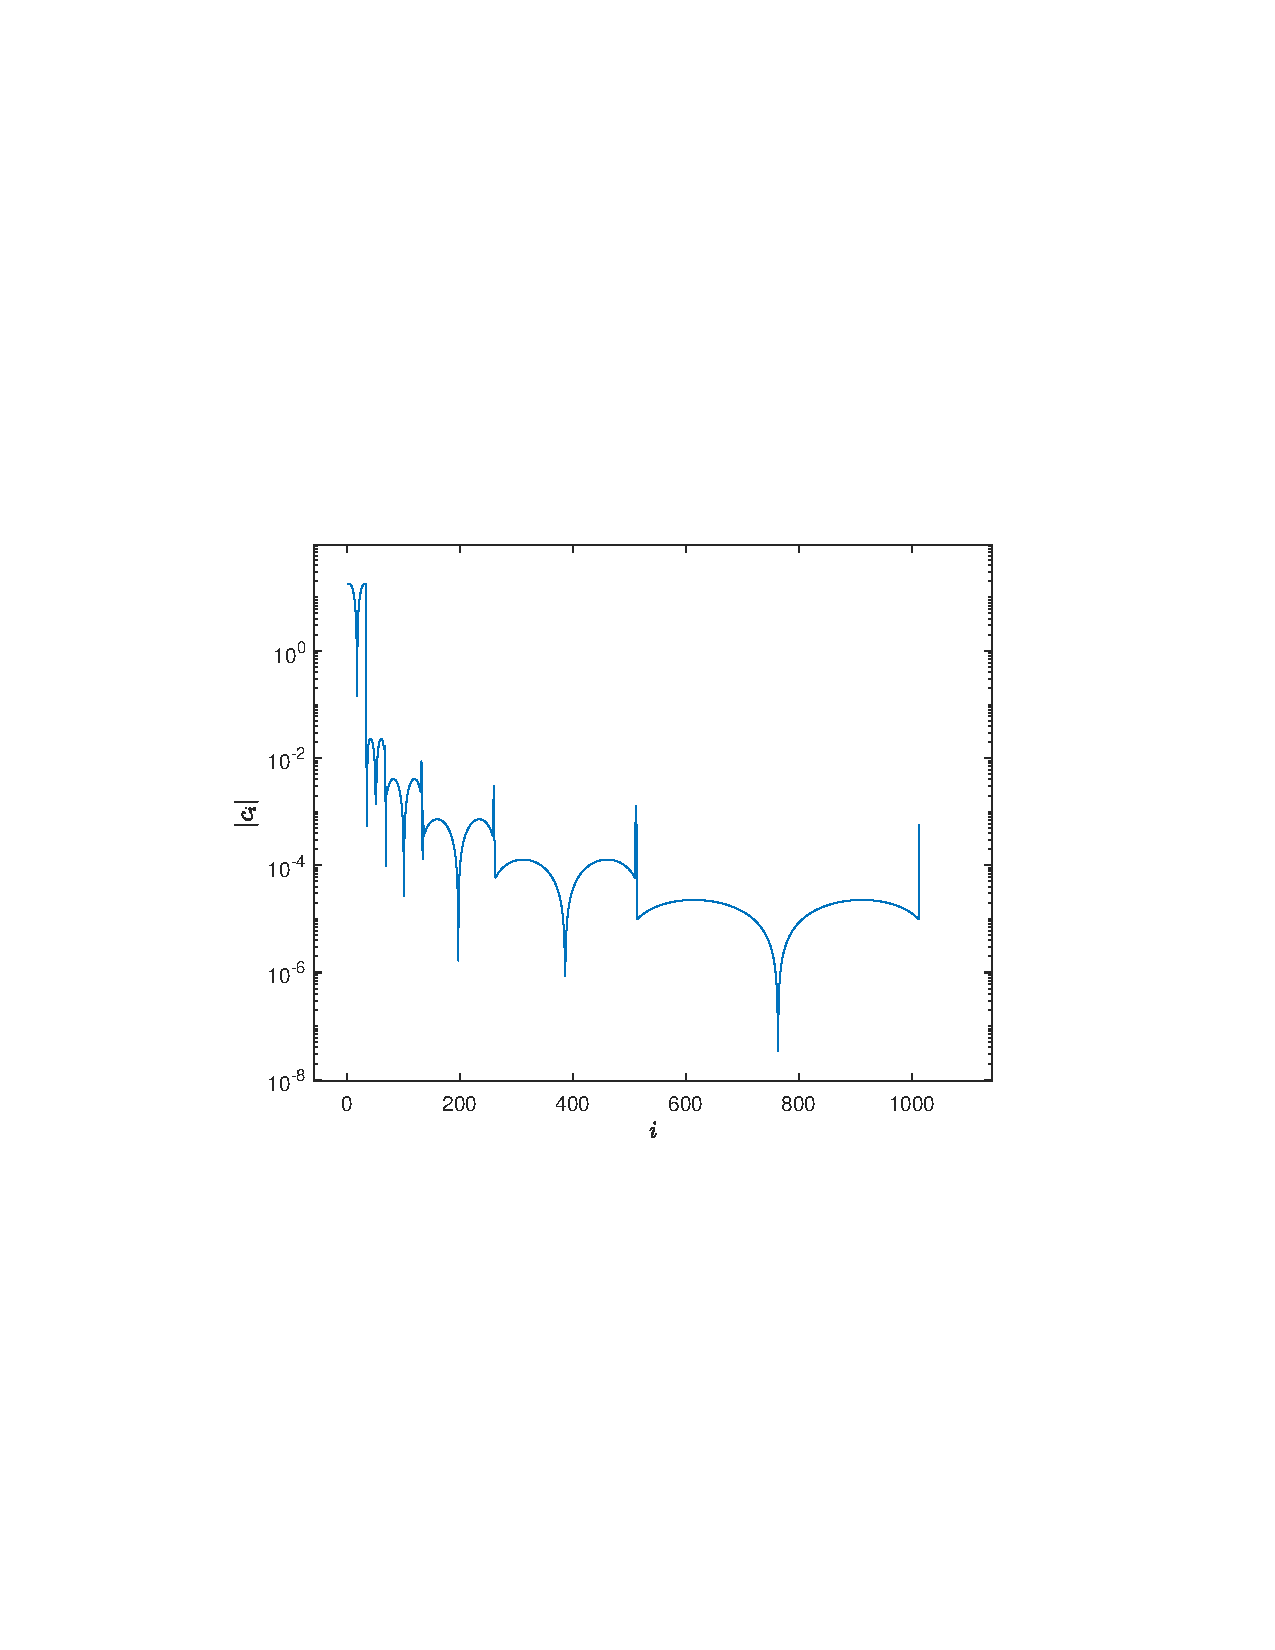
\includegraphics[trim={3.5cm 8cm 4cm 9cm},clip,width=0.7\textwidth]{Images/Coefficents.pdf}
	\caption{Coefficients of Wavelet transform (4 levels deep, using the Daubechies 2, $N=1000$ sample points, between $[-2,2]$}
	\label{fig:Coeff}
    \end{figure}

    We can see in \cref{fig:Coeff}, that the size of the coefficients decreases as $i$ increases. The meaning of this is that the coefficients of small size are of less importance to the reconstruction of the signal, and can be more easily effected by added noise.

    \subsubsection{Task 2.2}

    \subsubsection{Question 2.3}

    \subsection{Images with noise}

    \subsubsection{Task 2.4}

    \subsubsection{Question 2.5}

    \subsection{Using a redundant wavelet transform}

    \subsubsection{Task 2.6}

    \subsubsection{Question 2.7}

    \subsubsection{Question 2.8}

    \subsubsection{Task 2.9}

    \section{Wavelet-based inpainting}

    \subsection{An iterative algorithm}

    \subsubsection{Task 3.1}

    \subsubsection{Question 3.2}

    \subsubsection{Question 3.3}

    \subsubsection{Question 3.4}

 \end{document}